\documentclass{hfutpaper}
\usepackage[urlcolor=blue]{hyperref}
\usepackage{threeparttable}
\usepackage{setspace}
\usepackage{titlesec}
\usepackage{amsmath}
\usepackage{animate}
\usepackage{float}
\usepackage{listings}
\usepackage{wasysym}
\usepackage{makecell}
\usepackage{graphicx}
\usepackage{epstopdf}
\usepackage{listings}
\usepackage{booktabs}
\usepackage{indentfirst}
\usepackage{multirow}
\graphicspath{ {figure/} } 
\newcommand{\upcite}[1]{\textsuperscript{\textsuperscript{\cite{#1}}}}
\usepackage{fancyhdr}
\titleformat{\section}{\large \heiti}{\chinese{section}、}{0em}{}

\makeatletter
\newcommand{\figcaption}{\def\@captype{figure}\caption}
\newcommand{\tabcaption}{\def\@captype{table}\caption}
\makeatother
\setlength{\parindent}{2.45em}

\begin{document}
\begin{center}
\LARGE
  \textbf{萝卜分享会:简单但强大的MATLAB数据处理方式}\\
  \vspace{0.2em}
  \large
    许婷婷SA18168132,章坤SA18168226\\
    杜沈达SA18168163,刘淼SA18168215 \\ %姓名,学号,班级
    文献管理课第33组
  \end{center}
\rule[0.1\baselineskip]{\textwidth}{0.5pt}
\textbf{简 \ 介}\\
\large
本次萝卜分享会,我们组准备的是MATLAB数据可视化,主要介绍三大方面,第一是基础的MATLAB数据操作,包括读写和运算;第二是在MATLAB内进行画图,主要是介绍一些常用的绘图指令;第三是数据分析,主要介绍曲线拟合统计学工具箱的使用。
\\
\rule[0.1\baselineskip]{\textwidth}{0.5pt}
\section{数据获取}
\subsection{常用的数据读取}
\subsection*{从Excel表格读入}
只需要一条命令
\begin{lstlisting}[language=matlab]
data=xlsread('path\filename.xls(x)','Range');
\end{lstlisting}
这句命令说的意思就是把路径path下面的filename文件告诉MATLAB,要用读取Excel的方式xlsread读范围Range的数值。Range一般都写成A1:G15这样字的形式。

当然,除了读取还有写入,如果你做好了一个data矩阵的数据要写到Excel里面,只需要使用下面的命令,就可以把data里面的数据写到matlab里面了。
\begin{lstlisting}[language=matlab]
	xlswrite('path\filename.xls(x)',data);
\end{lstlisting}
\subsection*{txt文本读入数据}
有些软件处理之后的数据都是txt文本格式的,这时候就需要用文本读写指令来操作,读取也是一个指令完成。
\begin{lstlisting}[language=matlab]
	data=load('path\filename.txt')
\end{lstlisting}
这样子就可以加载一个文本文件的数据了,如果计算完数据要将其导出为文本文件数据,稍微有点麻烦。需要下面的指令完成。
\begin{lstlisting}[language=matlab]
[fid,errmsg]=fopen('txtTest.txt','wt');		
filename=fopen(fid);
fprintf(fid,'%f\t%f\n',data);
fclose(fid);
\end{lstlisting}
这个命令说的是先打开txtTest.txt的文本,用写命令打开,然后fid和errmsg是函数的输出参数,fid是一个整数,代表文件打开的状态,好像-1是表示不成功,这种都可以通过help去查看函数的具体用法,errmsg是代表函数的出错的信息,然后就把这个打开的文件名称告诉filename,这主要是在工作区可以看到文件夹名字,然后是核心指令fprintf把data输出到fid也就是文件里面,data的数据分两列写入文件,用tab隔开,之后再关闭文件。其实这个东西有点复杂了,一般把数据输出到Excel就够了可以发给别人看了,所以这个写入txt我也很少用到。值得说明一下的是,MATLAB的写函数的方式也就是这样子,其中function是关键字,[]里面的是输出的参数,FuncName是自定义函数的名称,()里面的是输入的参数。
\begin{lstlisting}[language=matlab]
function [outPara1,outPara2,...]=FuncName(inPara1,inPara2,...)
end
\end{lstlisting}
\subsection{总结}
主要就是讲了两个读取数据的方式,其中与Excel联合使用应该是比较常用并且实用的,命令也比较简单强大,txt一般在一些软件处理完输出一些参数可能会存入文本文件,这时候也需要用到,但是没事把数据写到txt文件再给别人看我还没有做过这样的事情。\blacksmiley
\section{数据计算和可视化}
数据计算就通过几个例子来说怎么做的吧,正好算完的数据可以用来画图,这也是很顺便的一件事情。
\section*{计算器计算}
要求:计算$12.5+\sqrt{3^2+4^2}+cos(\frac{\pi}{3})+3^5+2^3$

代码:
\lstinputlisting[language={MATLAB},
numbers=left, numberstyle={\normalsize },	commentstyle=\color{red!50!green!50!blue!50}, 
frame=shadowbox, rulesepcolor=\color{red!20!green!20!blue!20}]
{code/normalCalcu.m}

分析:上面的代码也就跟普通的计算器差不多,唯一要说明的是两个函数,一个是sqrt(x),一个是power(x,y)。sqrt(x)的x也就是要计算的表达式,把它写进括号也就是写进根号里面的意思,power(x,y)代表的是$x^y$,也就是跟普通的写$x^y$没什么区别,一般都用x\^{}y这样的形式,在帮助文档中可以看到说C = power(A,B) 是执行 A.\^{}B的替代方法, 但很少使用,所以一般用x\^{}y就够了。它可以启用类的运算符重载。还有一点需要说明的是,在$\sin,\cos$等三角函数进行运算的时候,\underline{用的都是弧度制。}
\section*{函数画法}
\lstinputlisting[language={MATLAB},
numbers=left, numberstyle={\normalsize },	commentstyle=\color{red!50!green!50!blue!50}, 
frame=shadowbox, rulesepcolor=\color{red!20!green!20!blue!20}]
{code/simpPlot.m}
其中figure(2)是再建立一个窗口用来画图,xlabel('x');ylabel('y')用来对x,y轴打标注,title('xxx')用来写标题。

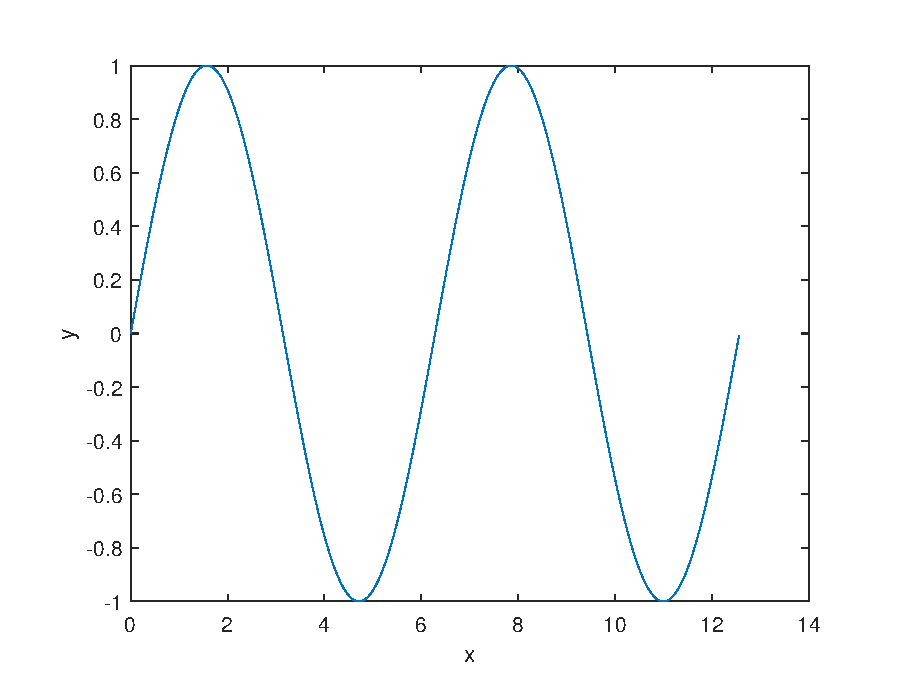
\includegraphics{figure/plot1.eps}
\figcaption{$y=sin(x)$}
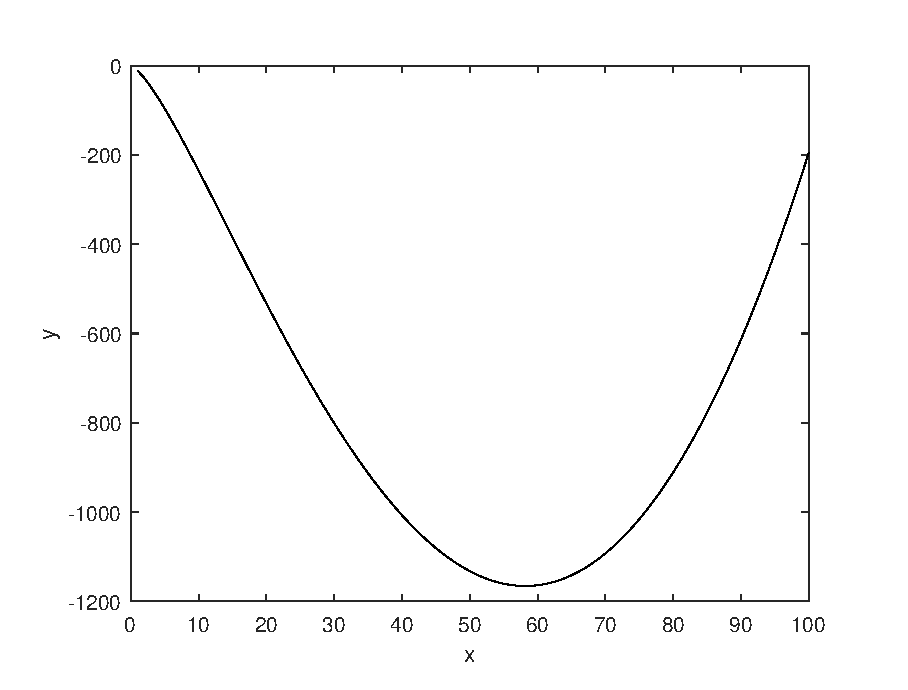
\includegraphics{figure/plot2.eps}
\figcaption{$y=x^2-2x+\sqrt{x}-x^{\frac{1}{3}}-10x^{1.5}$}

\section*{隐函数画法}
\lstinputlisting[language={MATLAB},
numbers=left, numberstyle={\normalsize },	commentstyle=\color{red!50!green!50!blue!50}, 
frame=shadowbox, rulesepcolor=\color{red!20!green!20!blue!20}]
{code/yinFun.m}

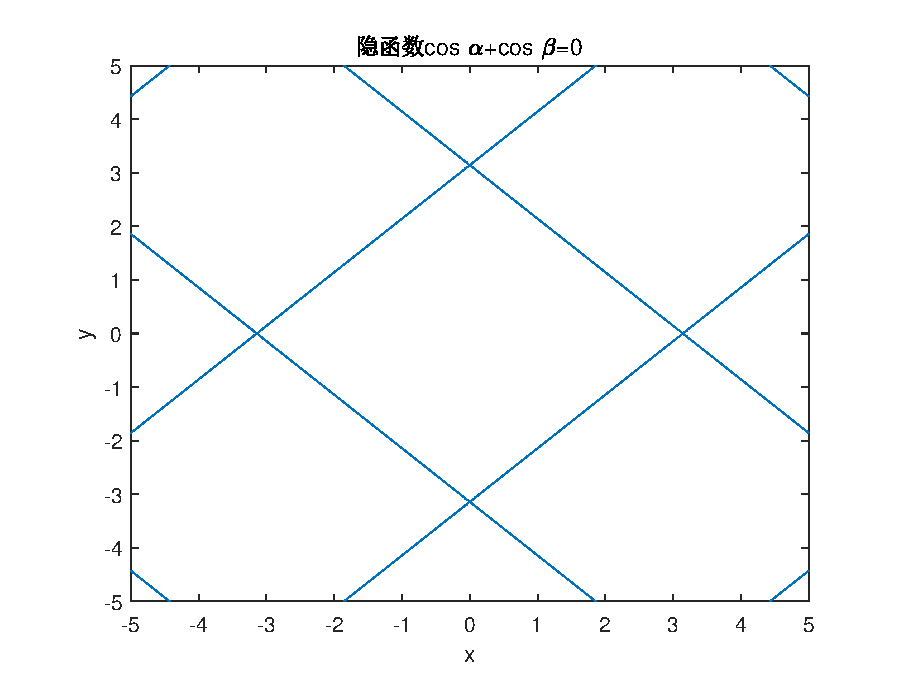
\includegraphics{figure/yinFunc}
\figcaption{隐函数$\cos \alpha+\cos \beta=0$}
\section*{子图画法}
\lstinputlisting[language={MATLAB},
numbers=left, numberstyle={\normalsize },	commentstyle=\color{red!50!green!50!blue!50}, 
frame=shadowbox, rulesepcolor=\color{red!20!green!20!blue!20}]
{code/subplotDemo.m}
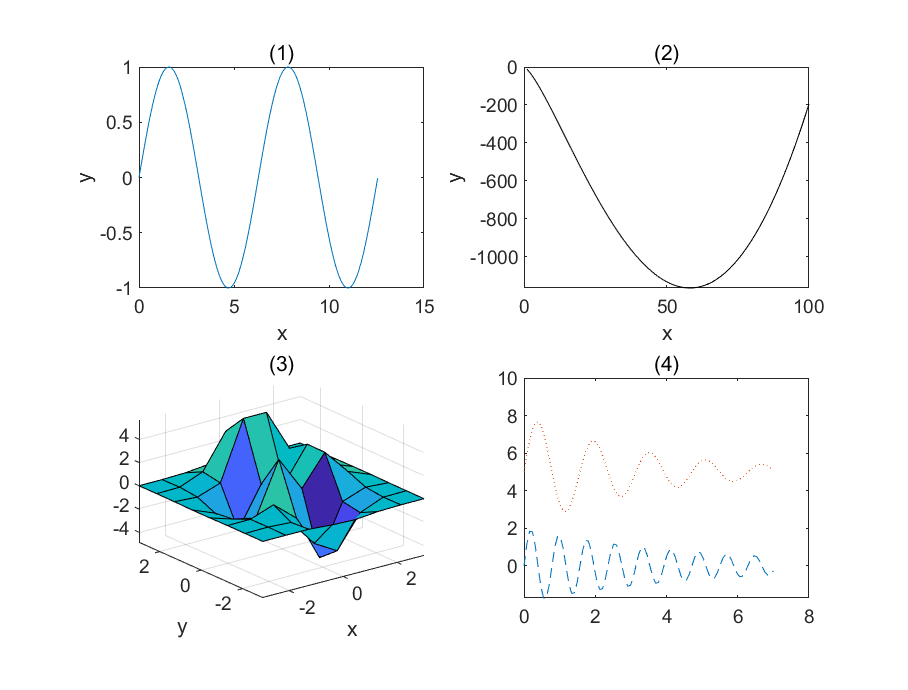
\includegraphics{figure/subplot}
\figcaption{子图画法}
\begin{center}
	(1)$y=\sin x$\\(2)$y=x^2-2x+\sqrt{x}-x^{\frac{1}{3}}-10x^{1.5}$\\
	(3)$peaks$函数\\(4)$y=2e^{-0.2x}\sin 8x$和$y=5+3e^{-0.3x}\sin 4x$
\end{center}
\section*{茎叶图和标注}
\lstinputlisting[language={MATLAB},
numbers=left, numberstyle={\normalsize },	commentstyle=\color{red!50!green!50!blue!50}, 
frame=shadowbox, rulesepcolor=\color{red!20!green!20!blue!20}]
{code/simpPlot2.m}
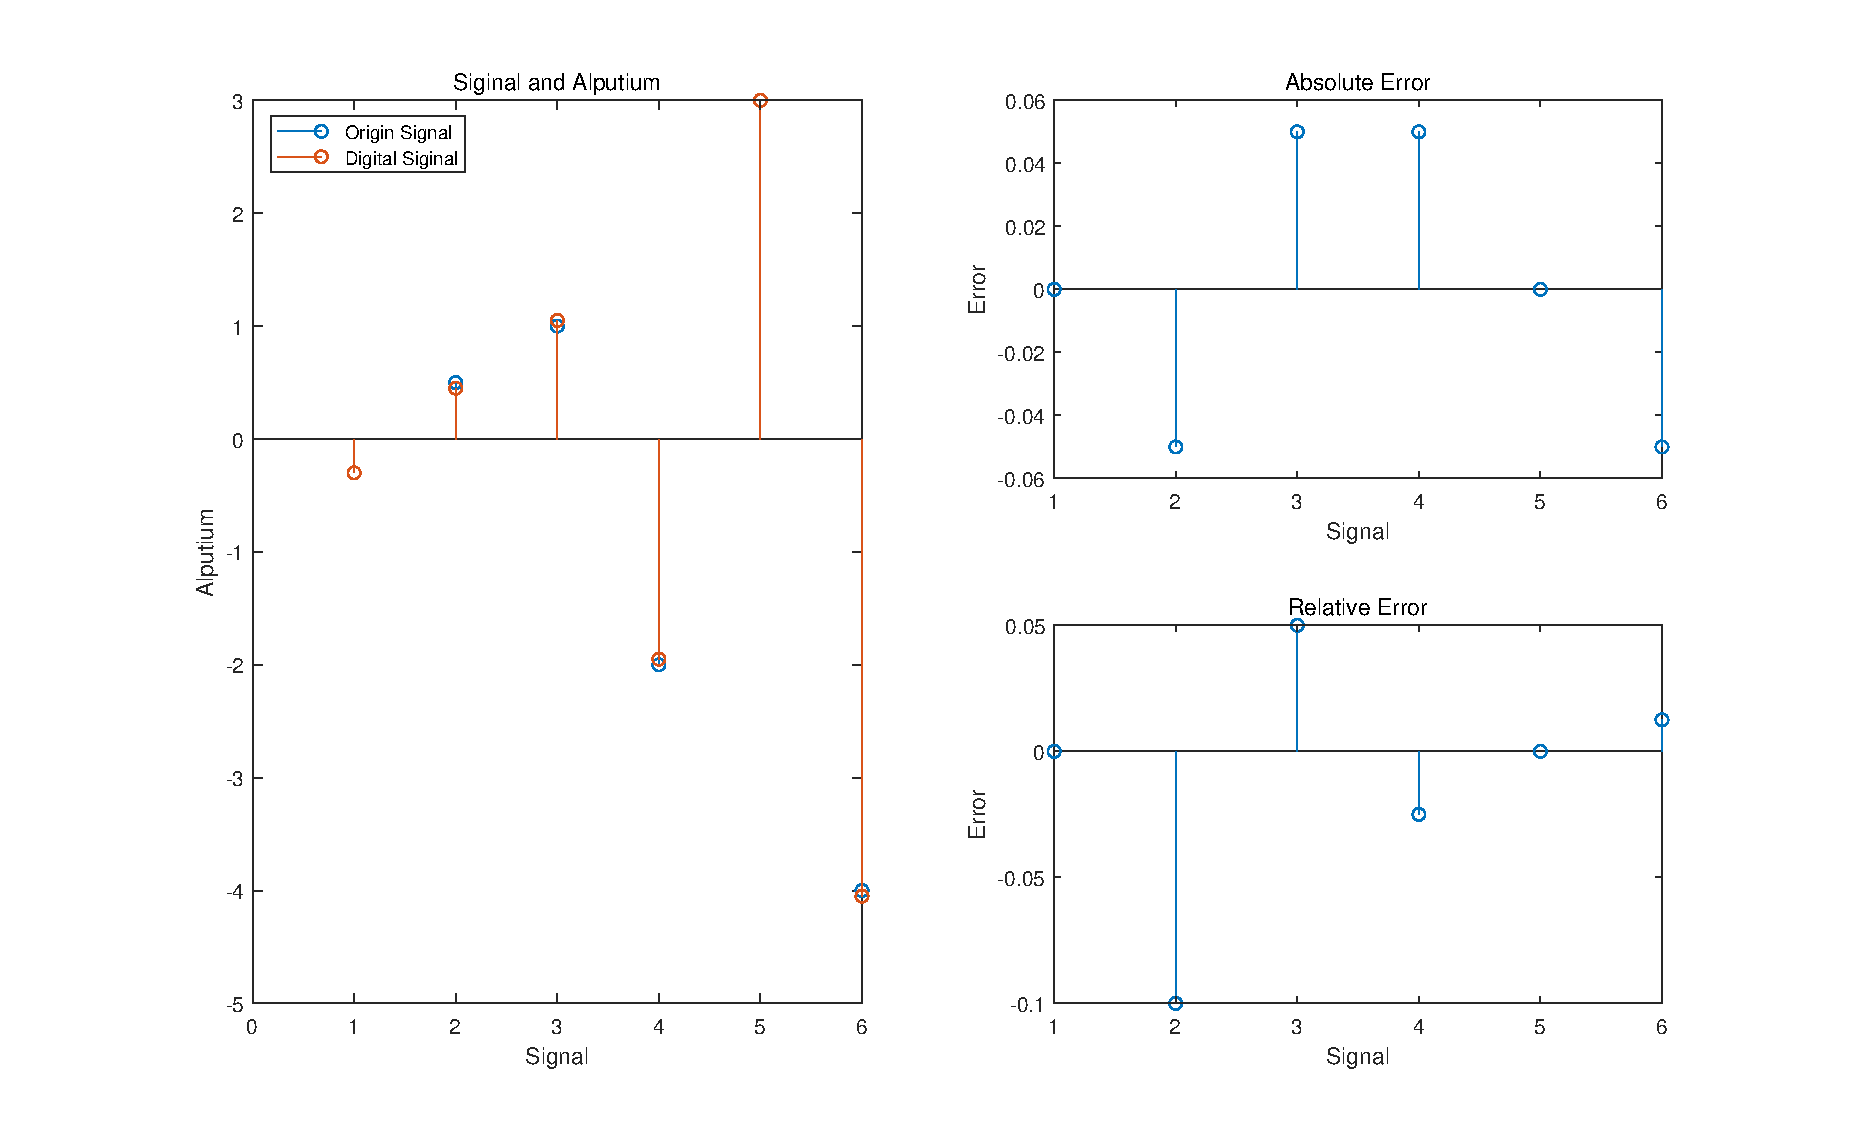
\includegraphics[width=17cm]{figure/stemAndLe}
\figcaption{茎叶图和标注}
\section*{双对数坐标轴}
\lstinputlisting[language={MATLAB},
numbers=left, numberstyle={\normalsize },	commentstyle=\color{red!50!green!50!blue!50}, 
frame=shadowbox, rulesepcolor=\color{red!20!green!20!blue!20}]
{code/loglogDemo.m}
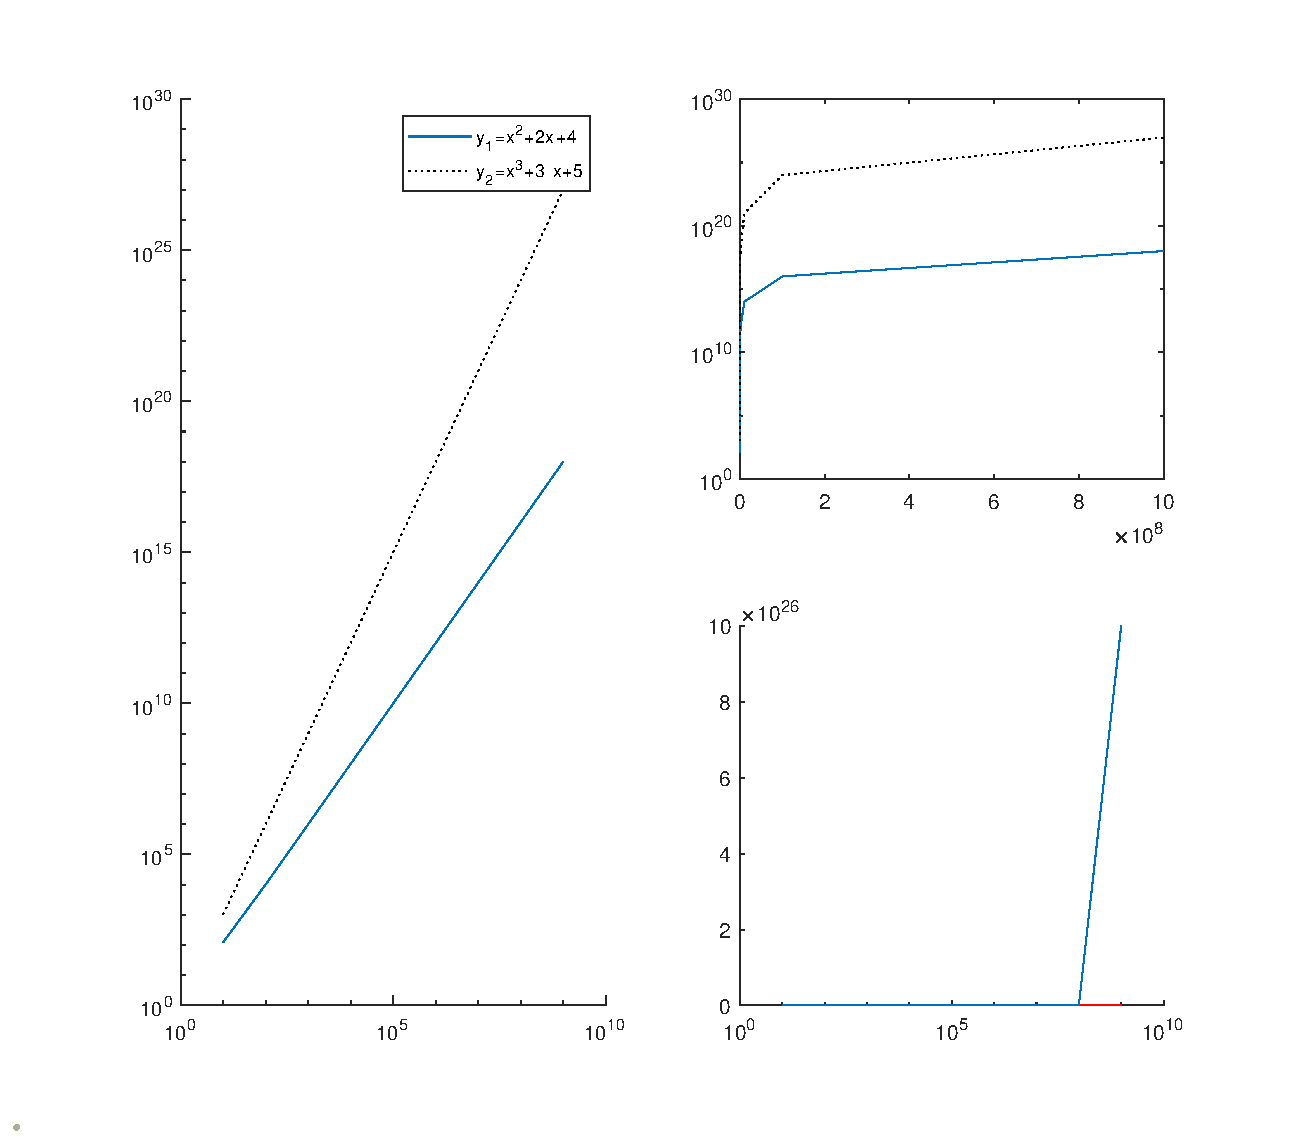
\includegraphics[width=18cm]{figure/loglog.eps}
\figcaption{双对数坐标绘图}
\section{函数表达式画图}
之前的plot命令都是根据点连线画出的曲线,如果不知道x的取值,那怎么画图?就用\underline{fplot}命令即可
\section*{fplot绘图}
\lstinputlisting[language={MATLAB},
numbers=left, numberstyle={\normalsize },	commentstyle=\color{red!50!green!50!blue!50}, 
frame=shadowbox, rulesepcolor=\color{red!20!green!20!blue!20}]
{code/fplotDemo.m}
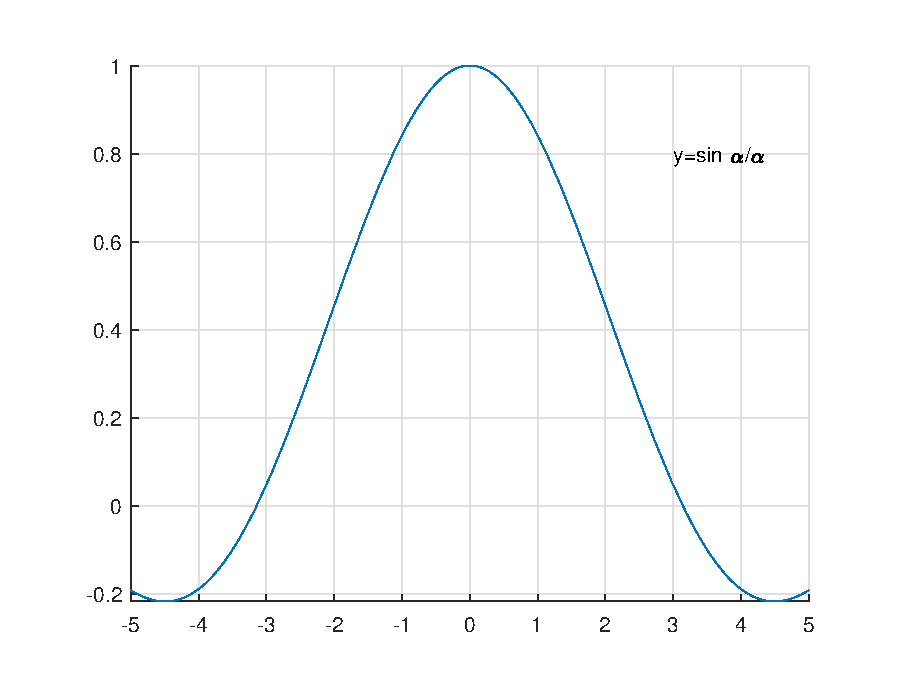
\includegraphics{figure/textAndFplot.eps}
\figcaption{text打标记和fplot画图}
\section*{交互绘图}
这个看图是看不出来什么的,要把代码放进MATLAB里面跑一下会比较好,大概适用于画出了某些函数,然后要写个标注,但是现在的标注很多都在图像窗口可以完成了,所以可能有些鸡肋吧。
\lstinputlisting[language={MATLAB},
numbers=left, numberstyle={\normalsize },	commentstyle=\color{red!50!green!50!blue!50}, 
frame=shadowbox, rulesepcolor=\color{red!20!green!20!blue!20}]
{code/ginDemo.m}
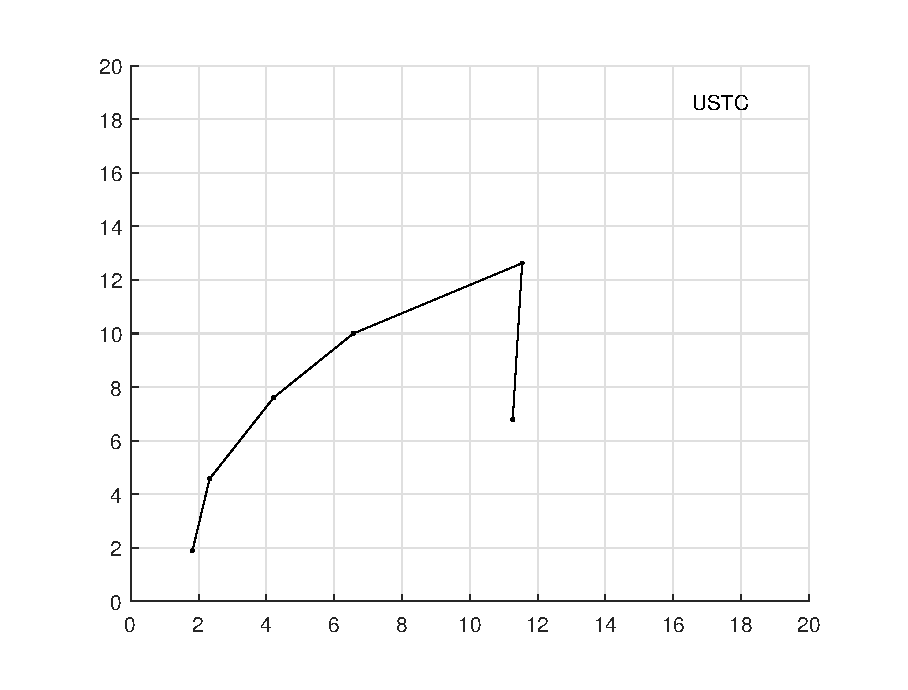
\includegraphics{figure/gin.eps}
\figcaption{交互绘图}
\section{常用作图}
\section*{柱状图}
\lstinputlisting[language={MATLAB},
numbers=left, numberstyle={\normalsize },	commentstyle=\color{red!50!green!50!blue!50}, 
frame=shadowbox, rulesepcolor=\color{red!20!green!20!blue!20}]
{code/barDemo.m}
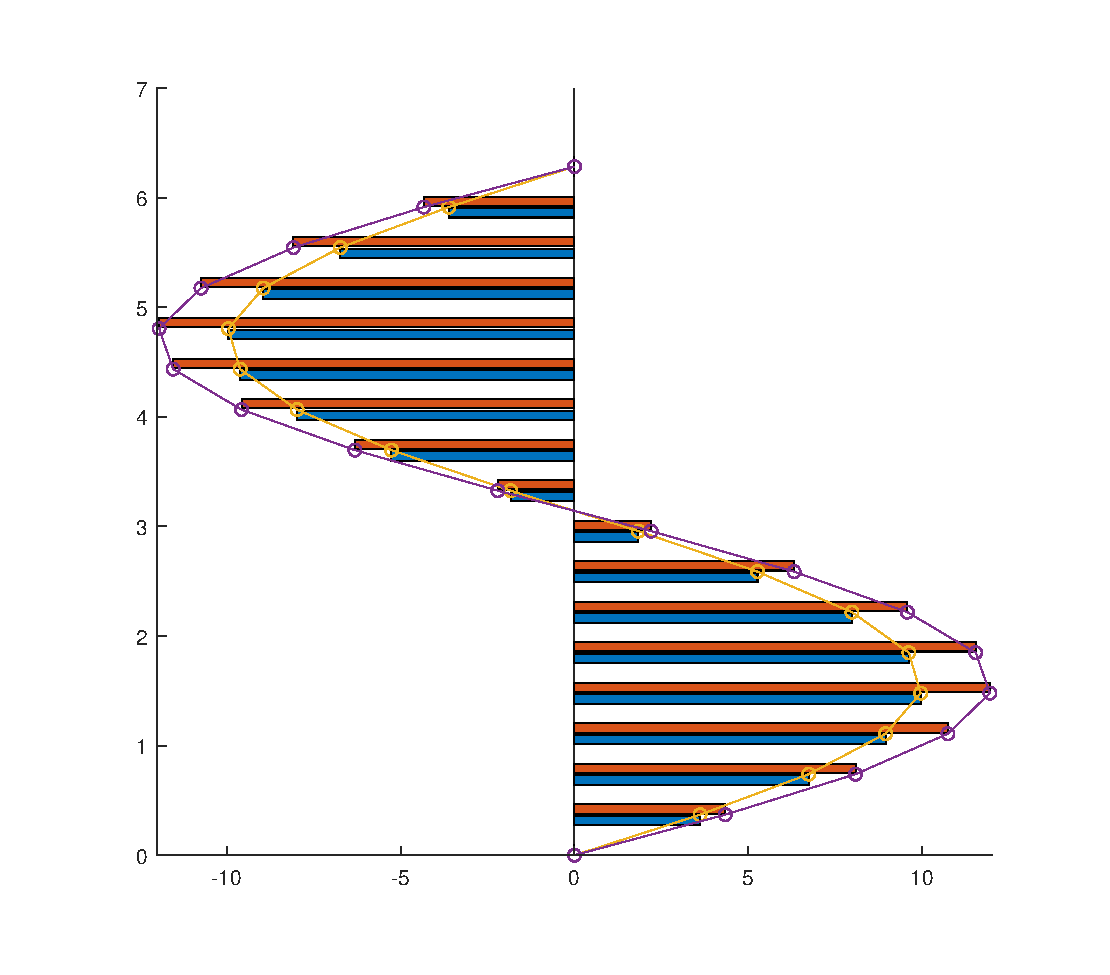
\includegraphics{figure/bar.eps}
\figcaption{水平柱状图绘制}
\section*{饼图绘制}
\lstinputlisting[language={MATLAB},
numbers=left, numberstyle={\normalsize },	commentstyle=\color{red!50!green!50!blue!50}, 
frame=shadowbox, rulesepcolor=\color{red!20!green!20!blue!20}]
{code/pieDemo.m}
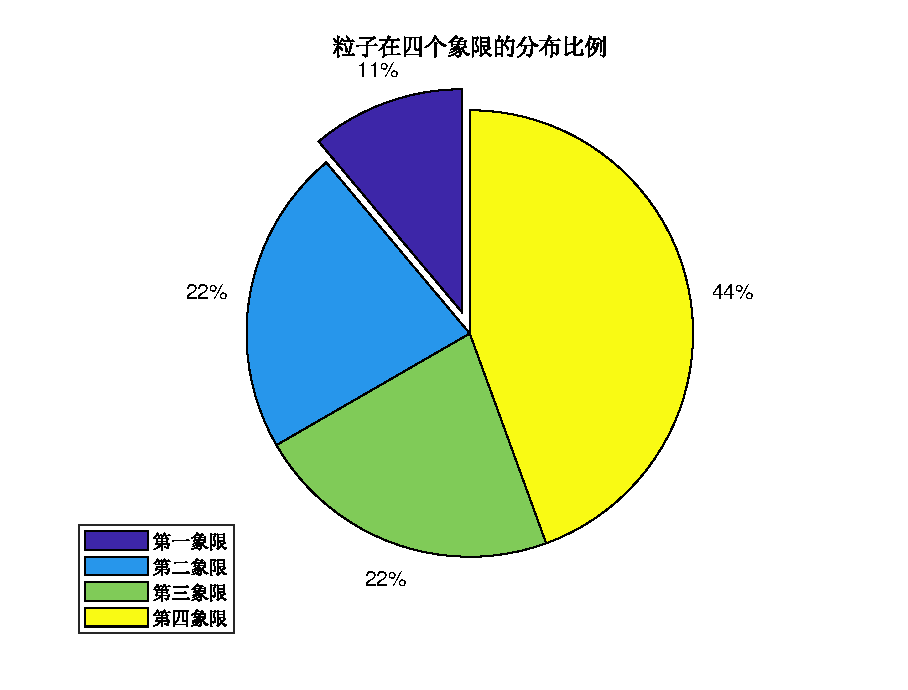
\includegraphics{figure/pie.eps}
\figcaption{饼图绘制}
\section*{彗星图}
这个也就是那种可以根据x取点一点一点走的图,emm,在这里还展示不了,MATLAB导出动图和pdf插入动图都比较麻烦,可以在MATLAB上面跑一下代码一下子就出来了,那个小圈就是轨迹出来的点。
\lstinputlisting[language={MATLAB},
numbers=left, numberstyle={\normalsize },	commentstyle=\color{red!50!green!50!blue!50}, 
frame=shadowbox, rulesepcolor=\color{red!20!green!20!blue!20}]
{code/comentDemo.m}
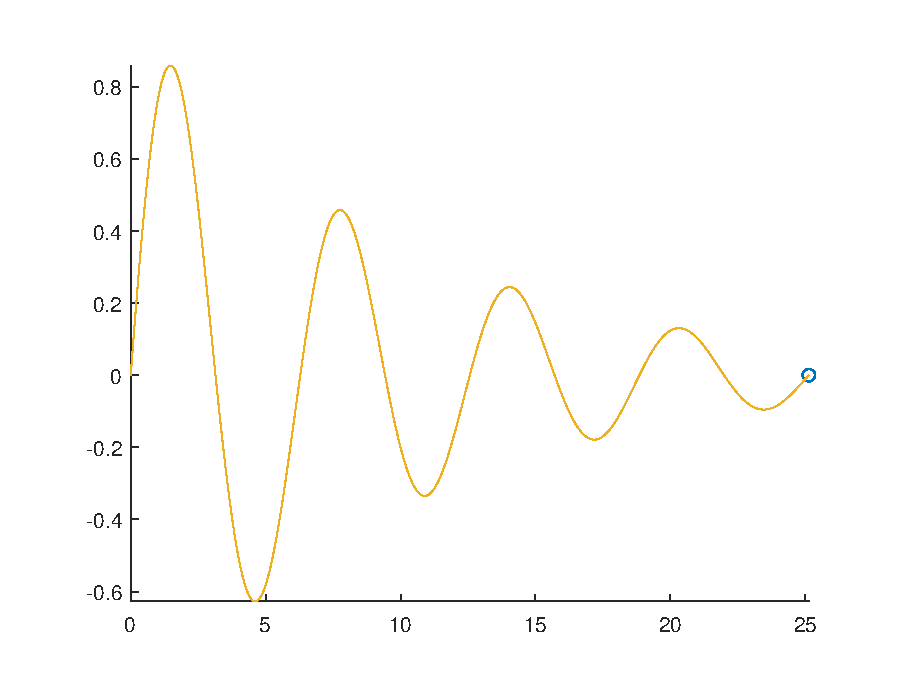
\includegraphics{figure/comet.eps}
\figcaption{彗星图(这里是静态的,要在MATLAB里面跑)}
\subsection*{其他绘图}
\lstinputlisting[language={MATLAB},
numbers=left, numberstyle={\normalsize },	commentstyle=\color{red!50!green!50!blue!50}, 
frame=shadowbox, rulesepcolor=\color{red!20!green!20!blue!20}]
{code/compassDemo.m}
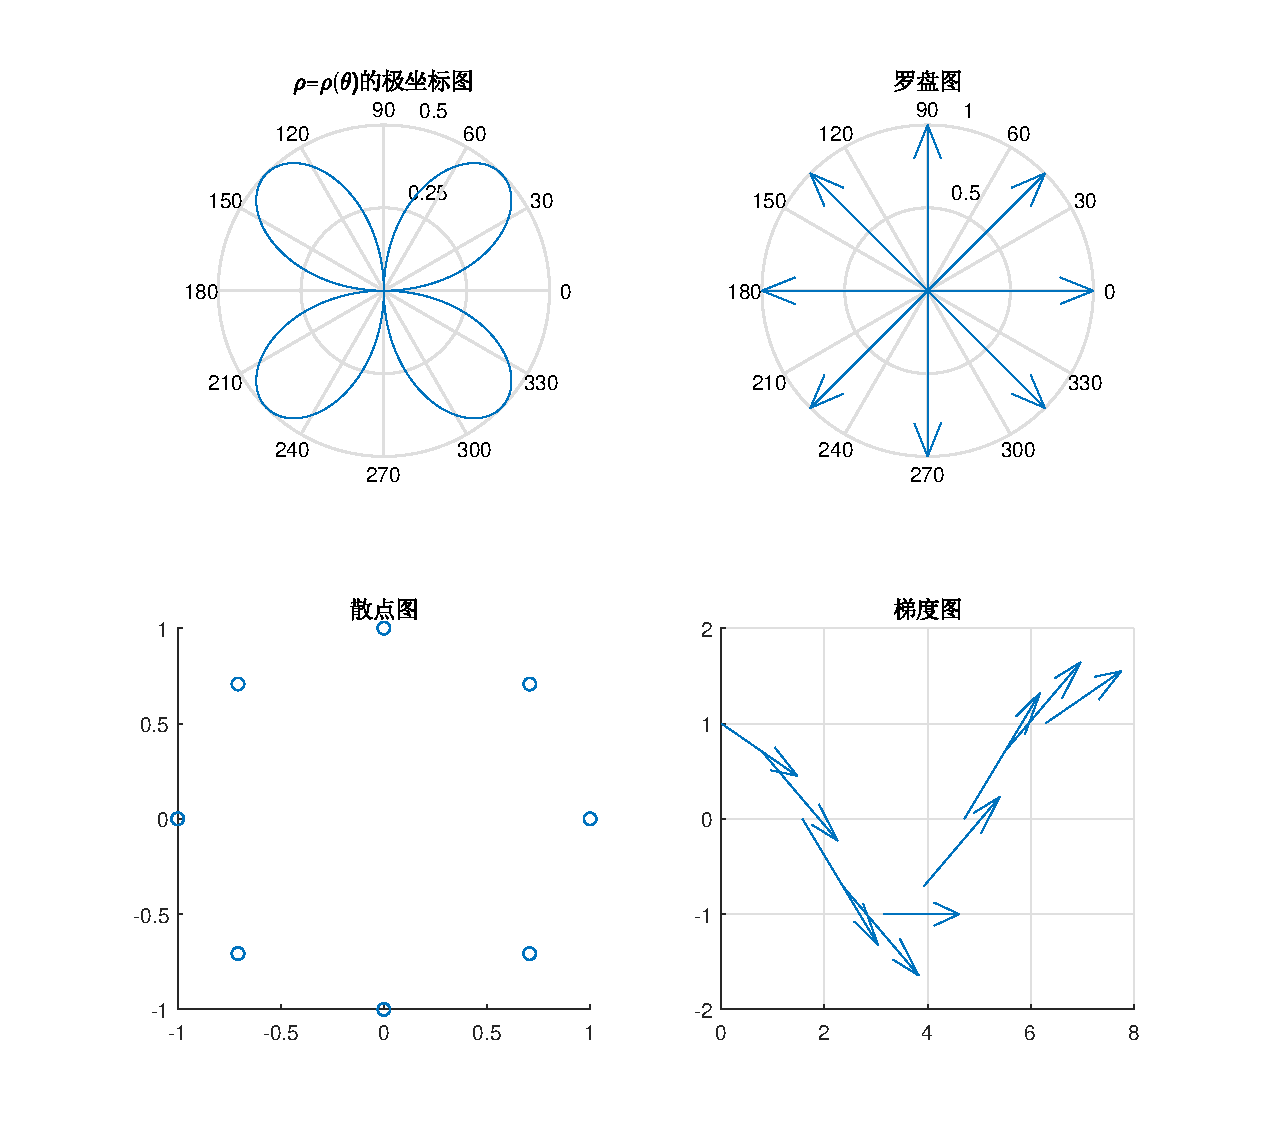
\includegraphics[width=18cm]{figure/plot3.eps}
\figcaption{(1)极坐标;(2)罗盘图;(3)散点图;(4)梯度图}
\section{三维图}
\section*{空间曲线}
\lstinputlisting[language={MATLAB},
numbers=left, numberstyle={\normalsize },	commentstyle=\color{red!50!green!50!blue!50}, 
frame=shadowbox, rulesepcolor=\color{red!20!green!20!blue!20}]
{code/plot33.m}
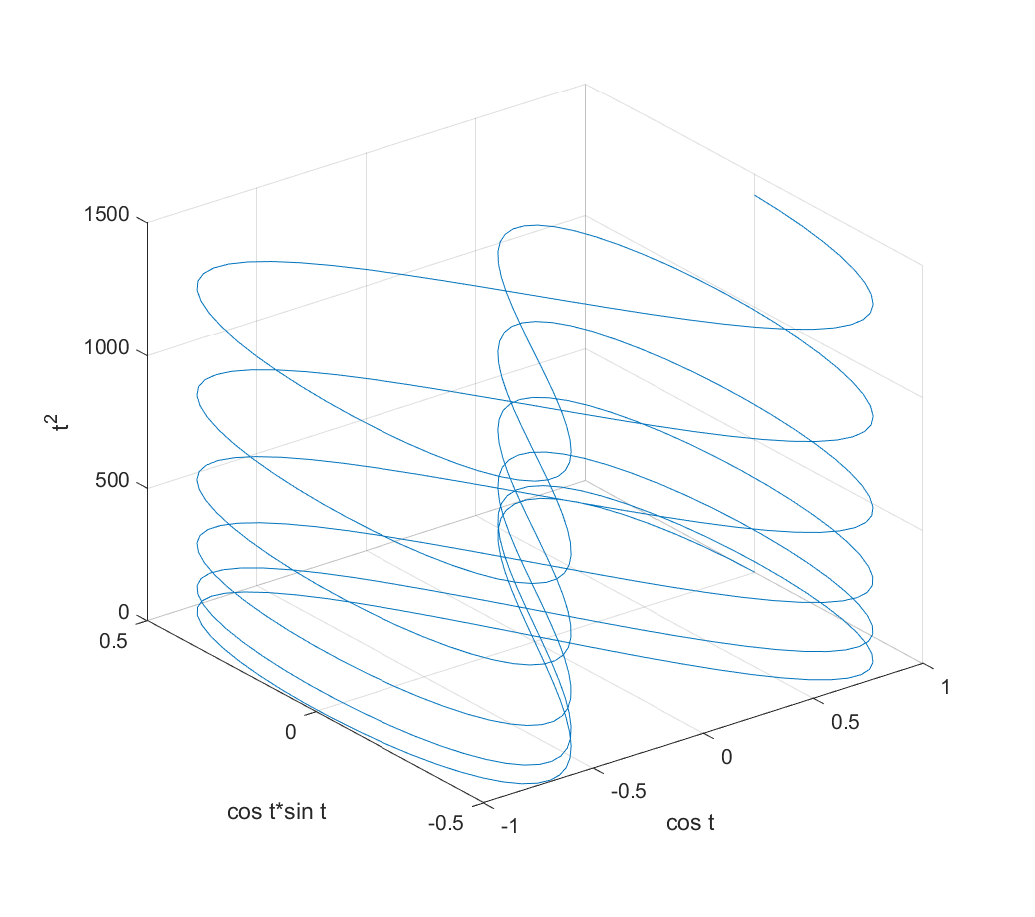
\includegraphics[width=18cm]{figure/plot33.eps}
\figcaption{空间曲线}
\section*{空间曲线切线}
\lstinputlisting[language={MATLAB},
numbers=left, numberstyle={\normalsize },	commentstyle=\color{red!50!green!50!blue!50}, 
frame=shadowbox, rulesepcolor=\color{red!20!green!20!blue!20}]
{code/d333.m}
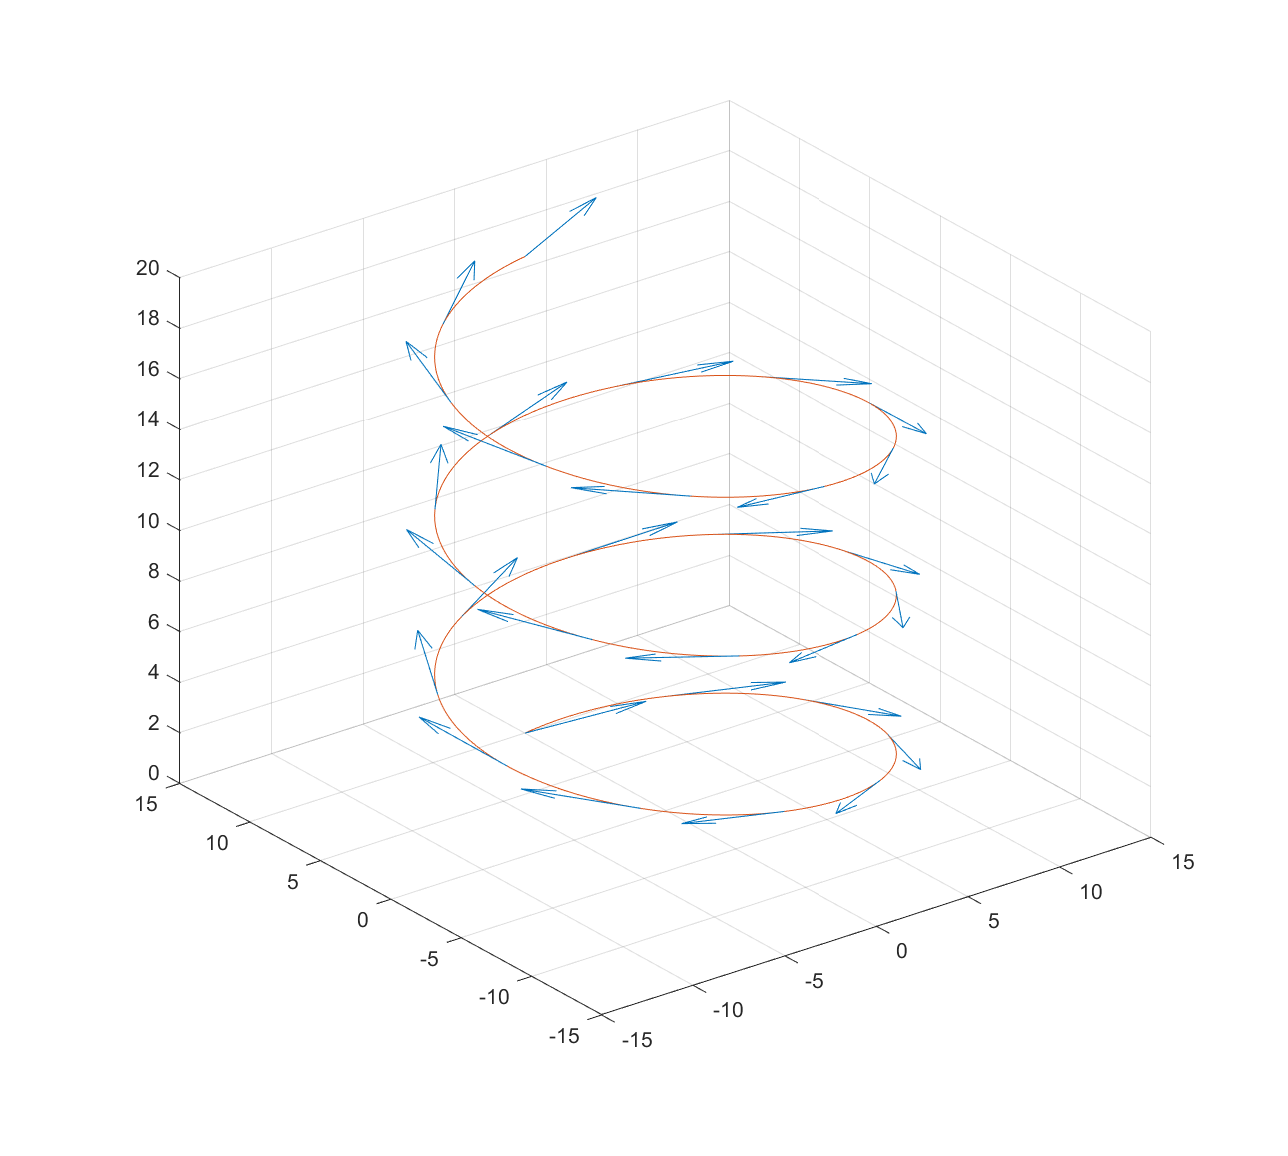
\includegraphics[width=18cm]{figure/d333.eps}
\figcaption{空间曲线切线}

\section*{三维曲面}
\lstinputlisting[language={MATLAB},
numbers=left, numberstyle={\normalsize },	commentstyle=\color{red!50!green!50!blue!50}, 
frame=shadowbox, rulesepcolor=\color{red!20!green!20!blue!20}]
{code/d3.m}
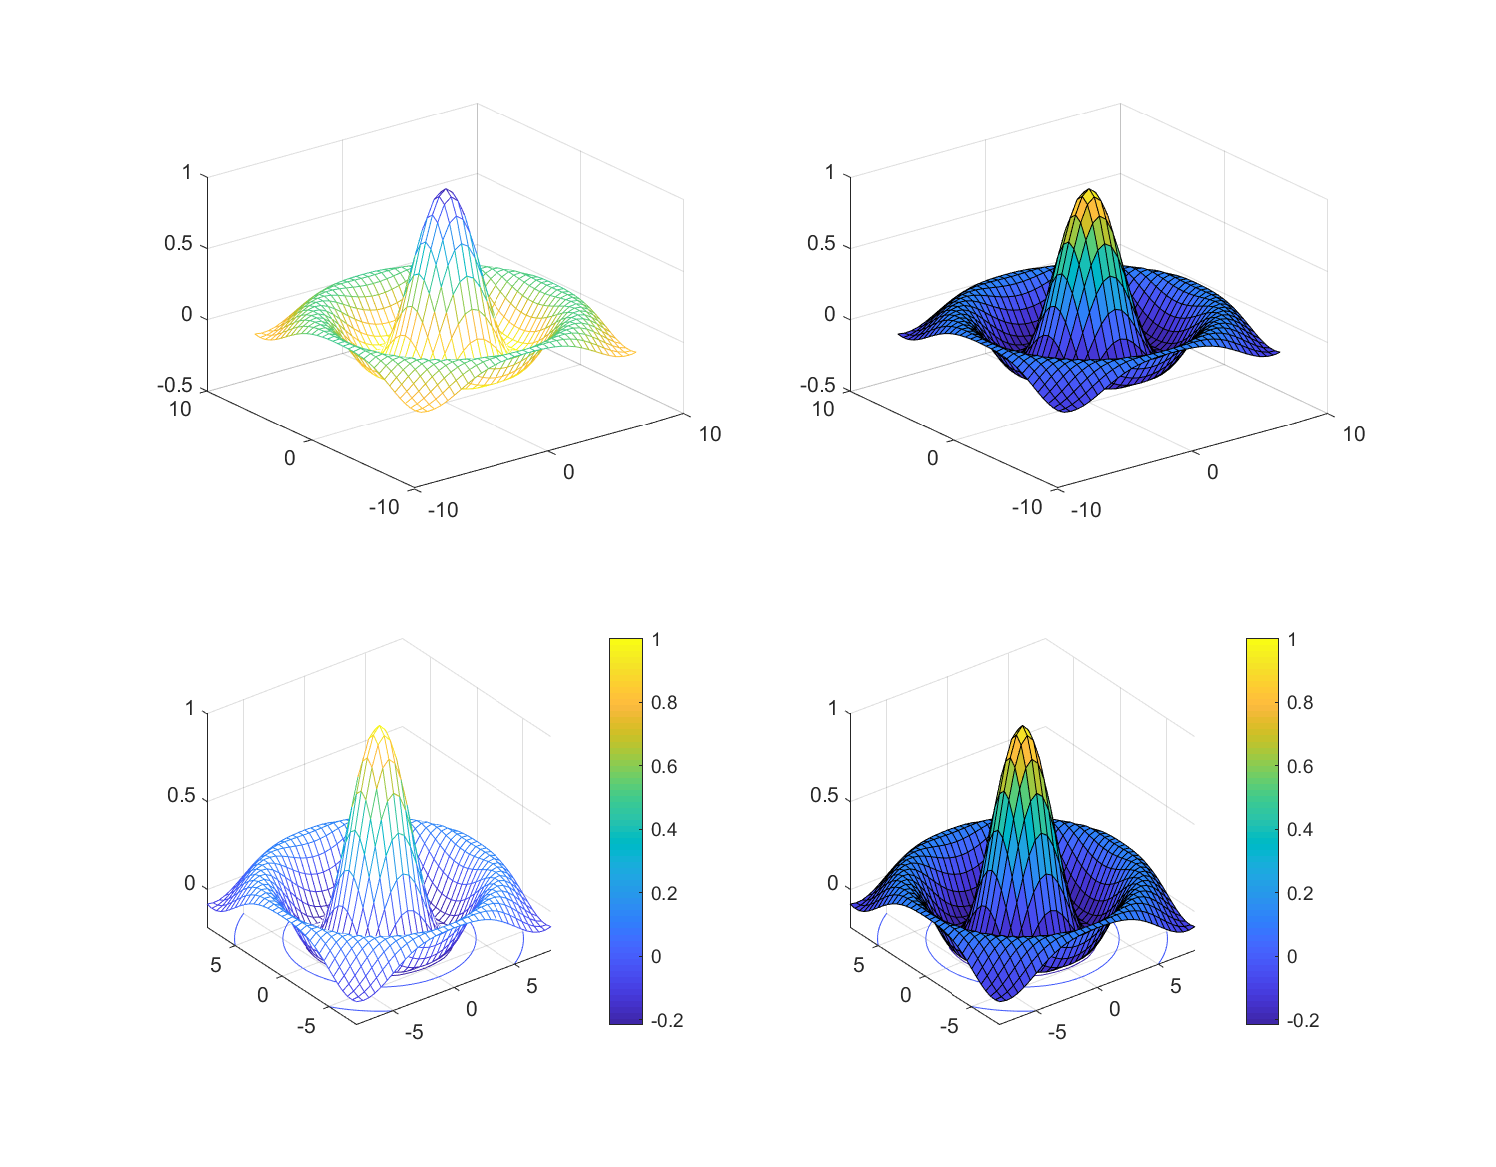
\includegraphics[width=18cm]{figure/MS.eps}
\figcaption{三维曲面}

\section*{几种其他的绘图命令}
\lstinputlisting[language={MATLAB},
numbers=left, numberstyle={\normalsize },	commentstyle=\color{red!50!green!50!blue!50}, 
frame=shadowbox, rulesepcolor=\color{red!20!green!20!blue!20}]
{code/sliceDemo.m}
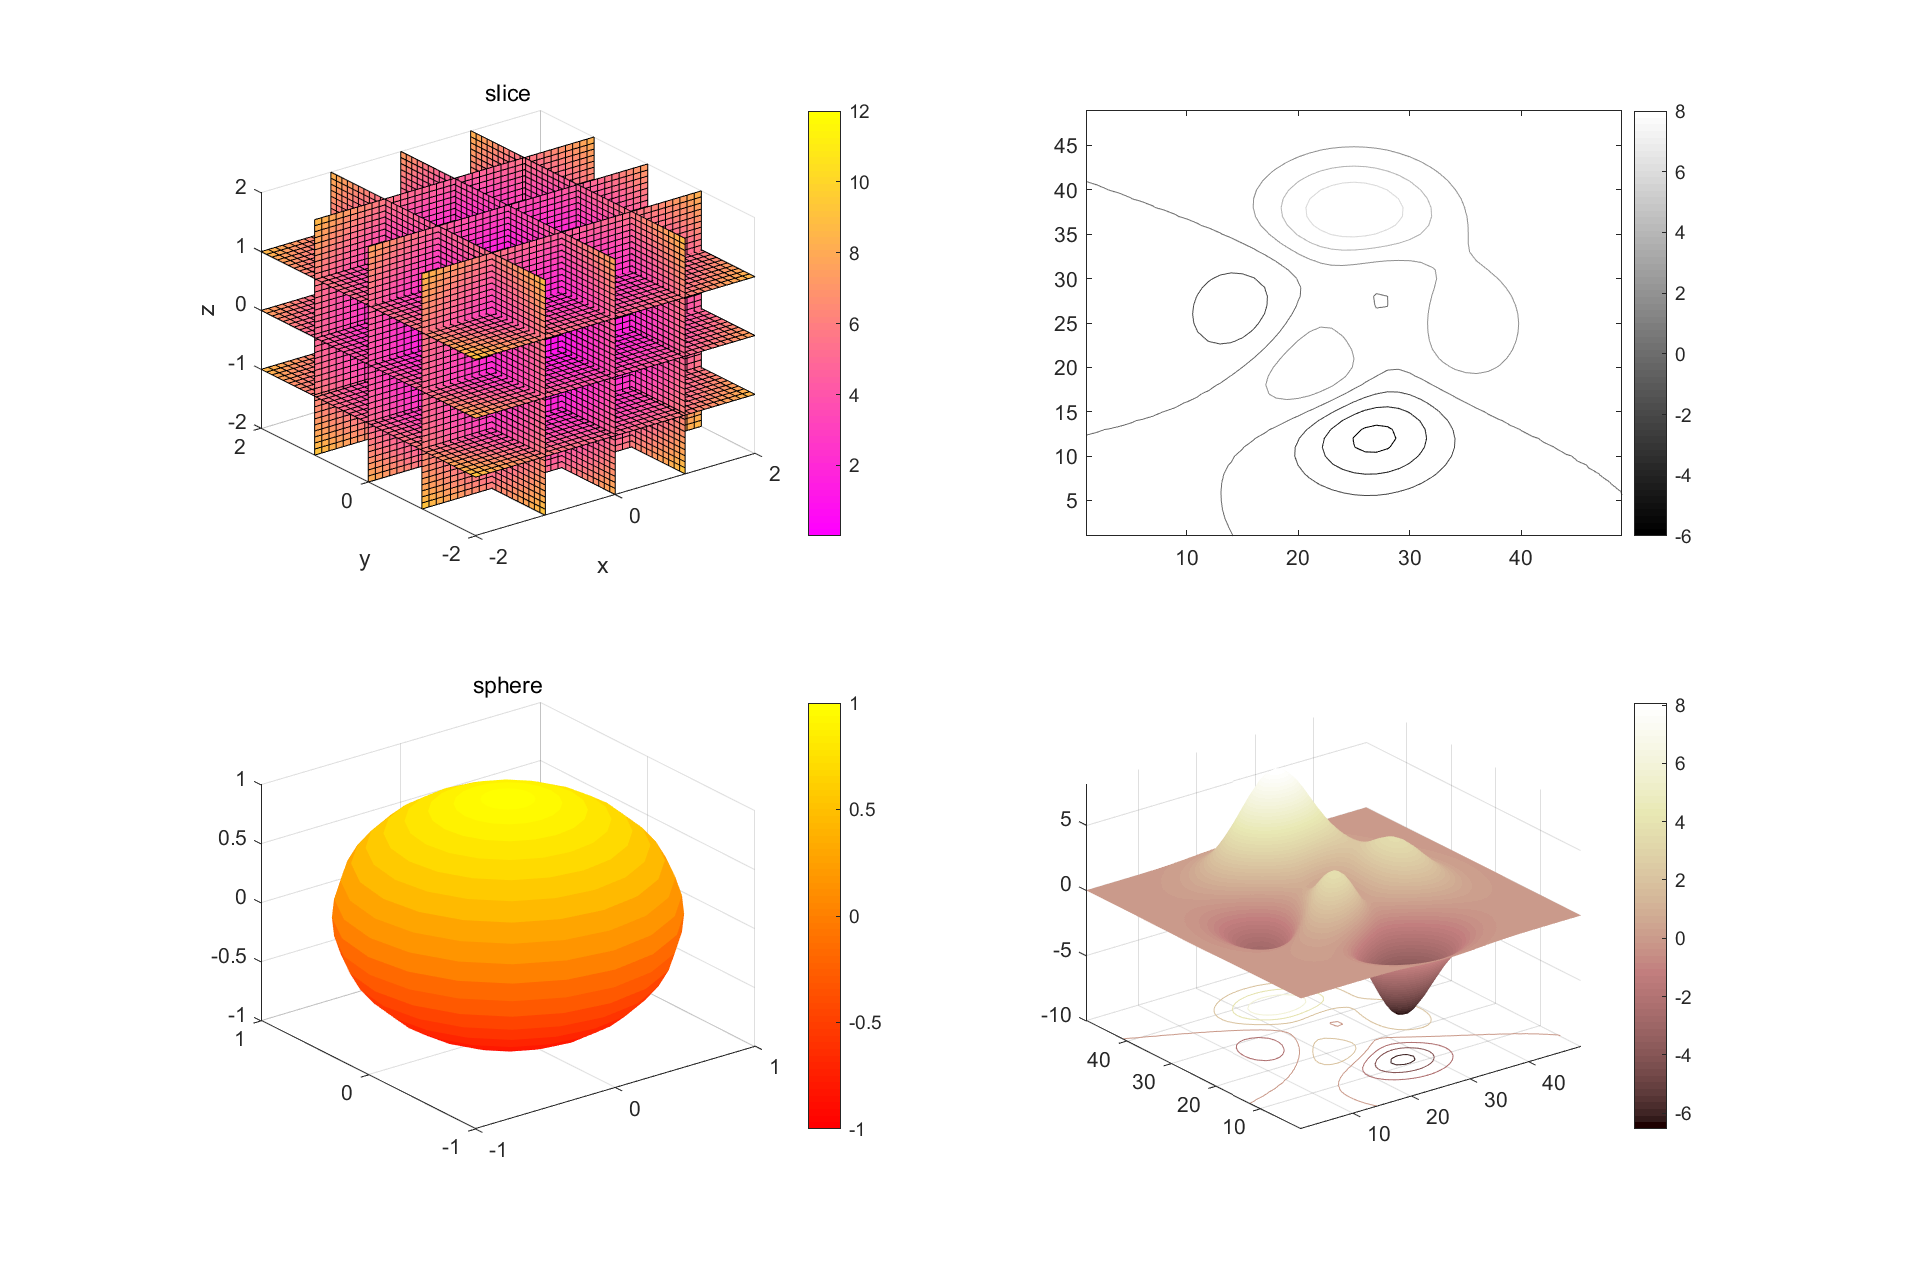
\includegraphics[width=18cm]{figure/d33.eps}
\figcaption{(1)slice;(2)contour;(3)colorbar;(4)surfc}
\section{几个有趣的例子}
\subsection*{莫比乌斯环}
\lstinputlisting[language={MATLAB},
numbers=left, numberstyle={\normalsize },	commentstyle=\color{red!50!green!50!blue!50}, 
frame=shadowbox, rulesepcolor=\color{red!20!green!20!blue!20}]
{code/mobiwusi.m}
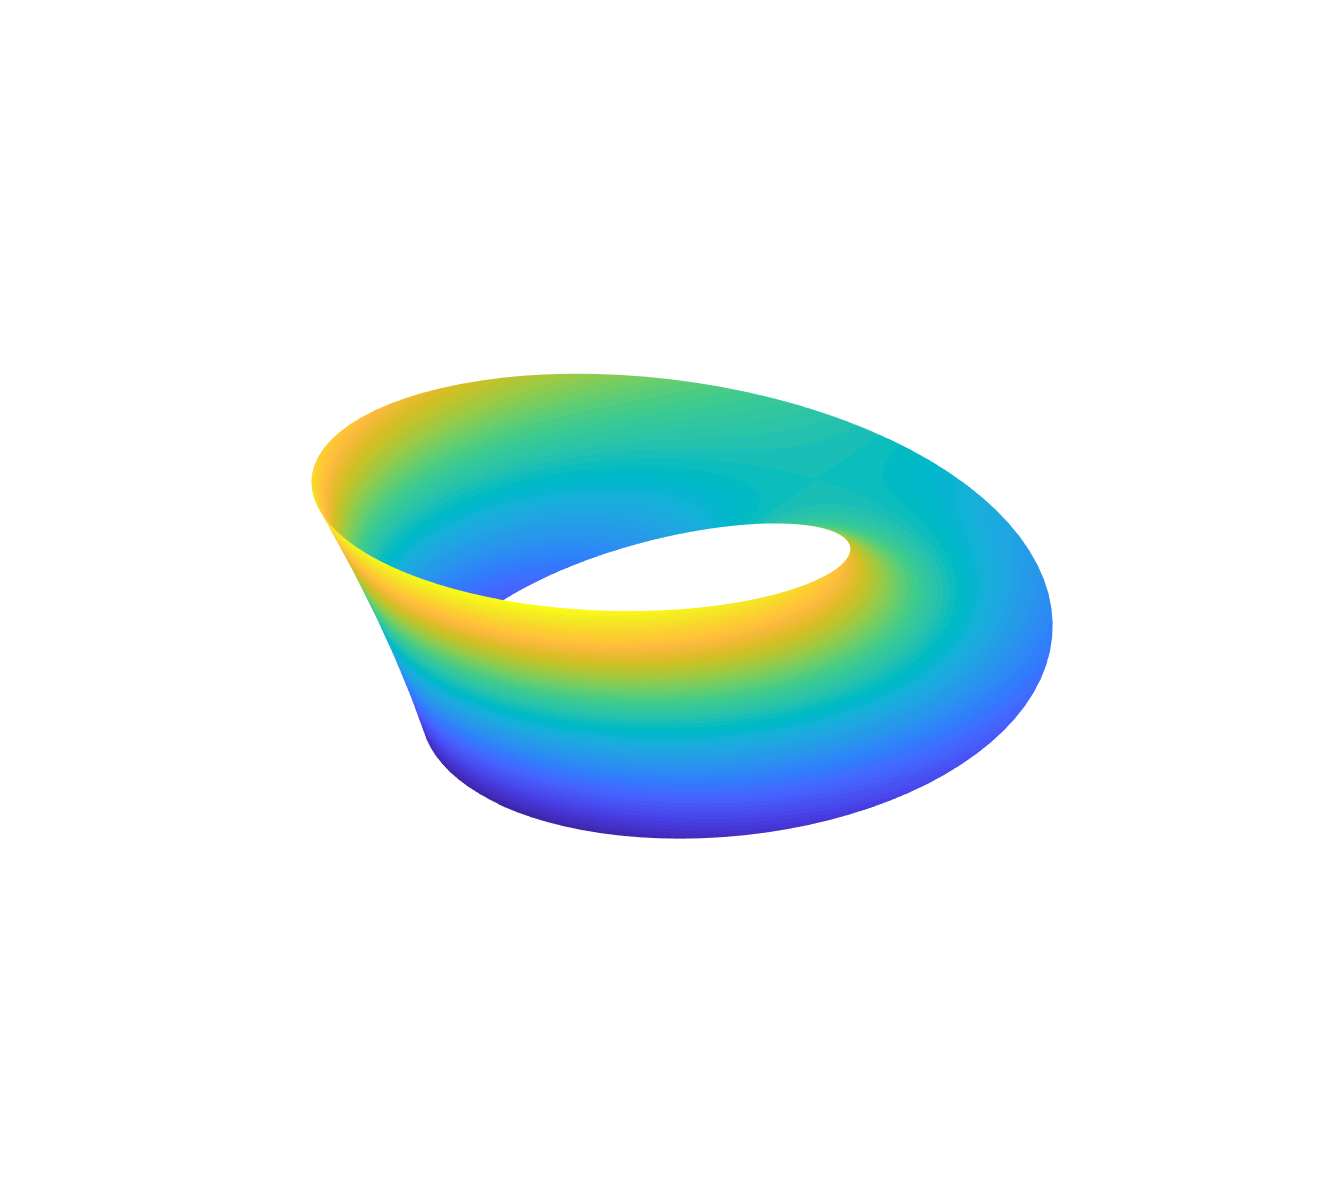
\includegraphics[width=18cm]{figure/mobiwusi.eps}
\figcaption{莫比乌斯环}
\section*{画一朵花}
\lstinputlisting[language={MATLAB},
numbers=left, numberstyle={\normalsize },	commentstyle=\color{red!50!green!50!blue!50}, 
frame=shadowbox, rulesepcolor=\color{red!20!green!20!blue!20}]
{code/mobiwusi.m}

\includegraphics[width=18cm]{figure/flower.eps}
\figcaption{花}
\section{统计作图}
\section*{四种常用的统计图}
下面介绍
主程序如下
\lstinputlisting[language={MATLAB},
numbers=left, numberstyle={\normalsize },	commentstyle=\color{red!50!green!50!blue!50}, 
frame=shadowbox, rulesepcolor=\color{red!20!green!20!blue!20}]
{code/StatisticCeshi.m}
下面是三个函数
\lstinputlisting[language={MATLAB},
numbers=left, numberstyle={\normalsize },	commentstyle=\color{red!50!green!50!blue!50}, 
frame=shadowbox, rulesepcolor=\color{red!20!green!20!blue!20}]
{code/sfpin.m}
\lstinputlisting[language={MATLAB},
numbers=left, numberstyle={\normalsize },	commentstyle=\color{red!50!green!50!blue!50}, 
frame=shadowbox, rulesepcolor=\color{red!20!green!20!blue!20}]
{code/fws.m}
\lstinputlisting[language={MATLAB},
numbers=left, numberstyle={\normalsize },	commentstyle=\color{red!50!green!50!blue!50}, 
frame=shadowbox, rulesepcolor=\color{red!20!green!20!blue!20}]
{code/dts.m}
\begin{center}
	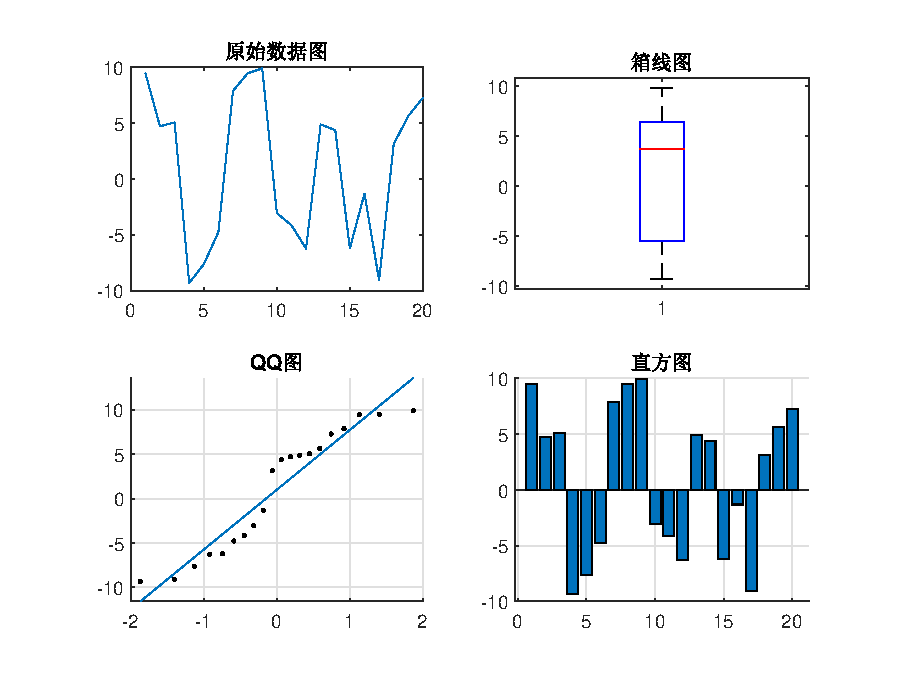
\includegraphics{figure/fourSF.eps}
	\figcaption{四种统计图}
	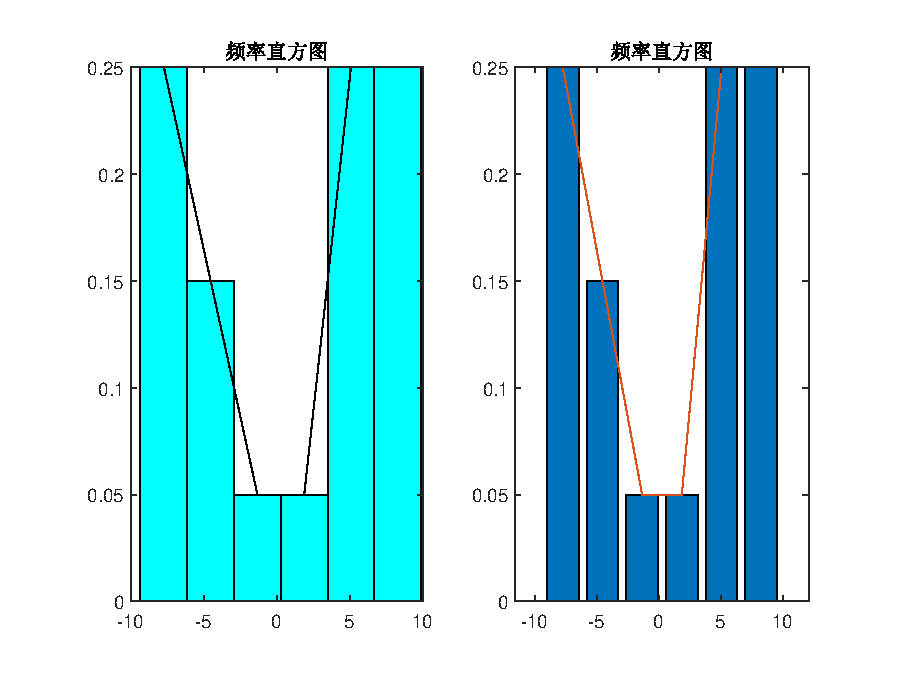
\includegraphics{figure/freBar.eps}
	\figcaption{两张频率直方图(使用不同的方法)}
\end{center}
\section*{拟合工具箱}
\begin{itemize}
\item Custom Equations:用户自定义的函数类型;
\item Exponential:指数逼近,有2种类型, $ae^{bx},ae^{bx}+ce^{dx}$;
\item Fourier:傅立叶逼近,有7种类型,基础型是 $a_0+a_1\cos {xw}+b_1\sin {xw}$;
\item Gaussian:高斯逼近,有8种类型,基础型是 $a_1e^{-(\frac{x-b_1}{c_1})^2}$;
\item Interpolant:插值逼近,有4种类型,linear,nearest,neighbor,cubic,spline,shape-preserving;
\item Polynomial:多形式逼近,有9种类型,linear ~、quadratic ~、cubic ~、4-9th degree ~
\item Power:幂逼近,有2种类型,$ax^b ,ax^b + c$;
\item Rational:有理数逼近,分子、分母共有的类型是linear,quadratic,cubic,4-5th degree ,此外分子还包括constant型;
\item Smoothing Spline:平滑逼近,样条曲线;
\item Sum of Sin Functions:正弦曲线逼近,有8种类型,基础型是 $a_1\sin{b_1x + c_1}$
\item Weibull:只有一种,$abx^{b-1}e^{-ax^b}$
\end{itemize}

\section{小技巧}
\begin{itemize}
	\item 开始学的时候可以用实时脚本文件做编程,“所见即所得”,这是很好的方式;
	\item \underline{help}很强大,一定要善于使用;
	\item MATLAB很强大也很简单,有用到就去学,不必一个一个对着书上敲代码把例子一个一个过,要是想学可以看一下用了什么指令,调用格式是什么,然后自己写一个,这样子应该会学的快一点。
\end{itemize}
\end{document} 